\documentclass[aspectratio=169]{beamer}
\usetheme{default}
\usecolortheme{default}
\usefonttheme{professionalfonts}
\usepackage{booktabs}
\usepackage{graphicx}
\usepackage{lmodern}
\usepackage{xcolor}

\definecolor{accent}{RGB}{30, 60, 120}
\definecolor{accentlight}{RGB}{235, 240, 252}

\setbeamertemplate{navigation symbols}{}
\setbeamertemplate{footline}[frame number]
\setbeamercolor{frametitle}{fg=white, bg=accent}
\setbeamerfont{frametitle}{size=\large, series=\bfseries}
\setbeamertemplate{frametitle}[default][center]
\setbeamercolor{title}{fg=accent}
\setbeamercolor{subtitle}{fg=black!60}
\setbeamerfont{title}{size=\Large, series=\bfseries}
\setbeamercolor{block title}{bg=accent, fg=white}
\setbeamercolor{block body}{bg=accentlight}
\setbeamerfont{block title}{series=\bfseries}
\setbeamercolor{normal text}{fg=black!85}
\renewcommand{\arraystretch}{1.2}

\graphicspath{{../report/figures/}}

\title{\textbf{Text Classification in NLP}}
\subtitle{CMPE346 --- Group 2}
\author{Atakan Gül \and [Student 2] \and [Student 3]}
\date{June 5, 2026}

\begin{document}

%% ── Slide 1: Title ──────────────────────────────────────────
\begin{frame}
\titlepage
\end{frame}

%% ── Slide 2: Group Overview ─────────────────────────────────
\begin{frame}{Overview}
\textbf{Group task:} Text Classification \hfill \textbf{Metric:} Accuracy \& Weighted F1

\vspace{0.5cm}
\begin{tabular}{ll}
\toprule
\textbf{Student} & \textbf{Task} \\
\midrule
Atakan Gül    & Media Bias Detection in News \\
{[Student 2]} & {[Topic]} \\
{[Student 3]} & {[Topic]} \\
\bottomrule
\end{tabular}
\end{frame}

%% ── Slide 3: Models ─────────────────────────────────────────
\begin{frame}{Models}
\begin{block}{BiLSTM}
Bidirectional LSTM trained from scratch. Captures sequential context in both directions.
\end{block}
\begin{block}{BERT}
Transformer encoder pretrained via masked language modeling. Fine-tuned end-to-end. \texttt{bert-base-uncased}.
\end{block}
\begin{block}{RoBERTa}
Optimized BERT: removes next sentence prediction, uses dynamic masking and more data. \texttt{roberta-base}.
\end{block}
\end{frame}

%% ══════════════════════════════════════════════
%% ATAKAN
%% ══════════════════════════════════════════════

%% ── Slide 4: Atakan — Task & Dataset ────────────────────────
\begin{frame}{Atakan Gül — Media Bias Detection}
\textbf{Task:} Classify a news sentence as \textit{biased} or \textit{not biased}.

\vspace{0.4cm}
\textbf{Dataset: BABE} (Bias Annotations By Experts)
\begin{itemize}
    \item 4,121 expert-annotated news sentences from diverse outlets
    \item 3,121 train / 1,000 test — binary labels
\end{itemize}
\end{frame}

%% ── Slide 5: Atakan — Results & Analysis ────────────────────
\begin{frame}{Atakan — Results}
\begin{columns}
\column{0.42\textwidth}
\begin{tabular}{lcc}
\toprule
\textbf{Model} & \textbf{Acc.} & \textbf{F1} \\
\midrule
BiLSTM   & 0.656 & 0.651 \\
BERT     & 0.826 & 0.827 \\
RoBERTa  & \textbf{0.846} & \textbf{0.846} \\
\bottomrule
\end{tabular}

\vspace{0.4cm}
\begin{itemize}
    \item RoBERTa best: +19\% over BiLSTM
    \item BERT close behind — both benefit from pretraining
    \item BiLSTM struggles on subtle linguistic bias
\end{itemize}
\column{0.58\textwidth}
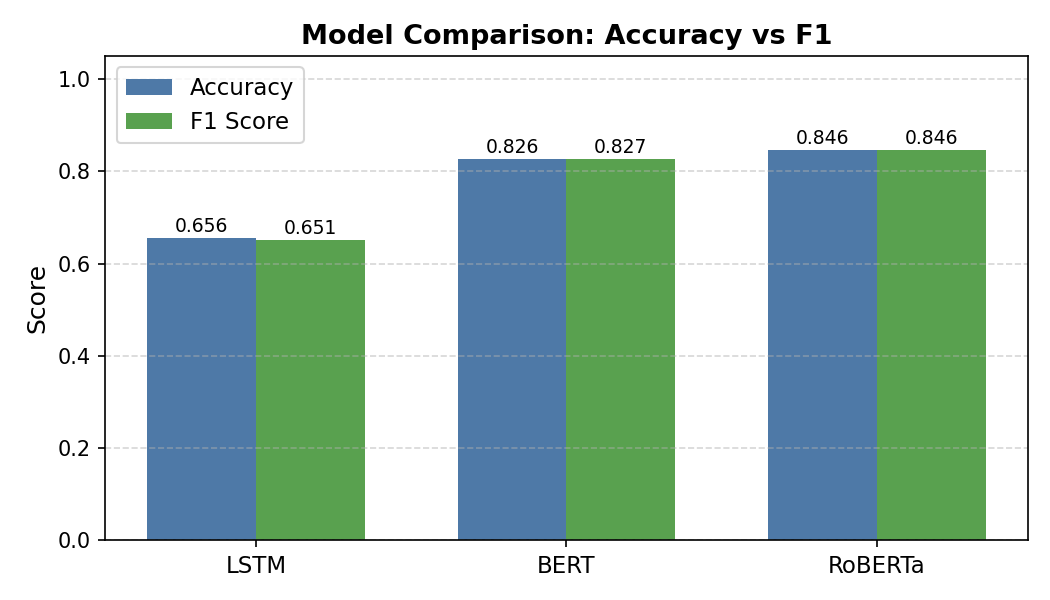
\includegraphics[width=\linewidth]{model_comparison.png}
\end{columns}
\end{frame}

%% ── Slide 6: Atakan — Conclusion ────────────────────────────
\begin{frame}{Atakan — Conclusion}
\begin{itemize}
    \item Media bias is a nuanced task — framing and tone, not facts
    \item Pretraining is critical: transformers extract subtle linguistic patterns BiLSTM cannot
    \item RoBERTa's optimized pretraining gives it a clear edge over BERT on this task
\end{itemize}
\end{frame}

%% ══════════════════════════════════════════════
%% STUDENT 2
%% ══════════════════════════════════════════════

%% ── Slide 7: Student 2 — Task & Dataset ─────────────────────
\begin{frame}{[Student 2] — [Topic]}
\textbf{Task:} [Description]

\vspace{0.4cm}
\textbf{Dataset:} [Name]
\begin{itemize}
    \item [Stats]
    \item [Train / test split]
\end{itemize}
\end{frame}

%% ── Slide 8: Student 2 — Results & Analysis ─────────────────
\begin{frame}{[Student 2] — Results}
\begin{columns}
\column{0.42\textwidth}
\begin{tabular}{lcc}
\toprule
\textbf{Model} & \textbf{Acc.} & \textbf{F1} \\
\midrule
BiLSTM   & — & — \\
BERT     & — & — \\
RoBERTa  & — & — \\
\bottomrule
\end{tabular}

\vspace{0.4cm}
\begin{itemize}
    \item [Key finding 1]
    \item [Key finding 2]
\end{itemize}
\column{0.58\textwidth}
\textit{[Figure or key observation]}
\end{columns}
\end{frame}

%% ── Slide 9: Student 2 — Conclusion ─────────────────────────
\begin{frame}{[Student 2] — Conclusion}
\begin{itemize}
    \item [Finding 1]
    \item [Finding 2]
    \item [Finding 3]
\end{itemize}
\end{frame}

%% ══════════════════════════════════════════════
%% STUDENT 3
%% ══════════════════════════════════════════════

%% ── Slide 10: Student 3 — Task & Dataset ────────────────────
\begin{frame}{[Student 3] — [Topic]}
\textbf{Task:} [Description]

\vspace{0.4cm}
\textbf{Dataset:} [Name]
\begin{itemize}
    \item [Stats]
    \item [Train / test split]
\end{itemize}
\end{frame}

%% ── Slide 11: Student 3 — Results & Analysis ────────────────
\begin{frame}{[Student 3] — Results}
\begin{columns}
\column{0.42\textwidth}
\begin{tabular}{lcc}
\toprule
\textbf{Model} & \textbf{Acc.} & \textbf{F1} \\
\midrule
BiLSTM   & — & — \\
BERT     & — & — \\
RoBERTa  & — & — \\
\bottomrule
\end{tabular}

\vspace{0.4cm}
\begin{itemize}
    \item [Key finding 1]
    \item [Key finding 2]
\end{itemize}
\column{0.58\textwidth}
\textit{[Figure or key observation]}
\end{columns}
\end{frame}

%% ── Slide 12: Student 3 — Conclusion ────────────────────────
\begin{frame}{[Student 3] — Conclusion}
\begin{itemize}
    \item [Finding 1]
    \item [Finding 2]
    \item [Finding 3]
\end{itemize}
\end{frame}

%% ══════════════════════════════════════════════
%% GROUP CONCLUSION
%% ══════════════════════════════════════════════

%% ── Slide 13: All Results ────────────────────────────────────
\begin{frame}{All Results}
\begin{tabular}{llcc}
\toprule
\textbf{Task} & \textbf{Model} & \textbf{Acc.} & \textbf{F1} \\
\midrule
\multirow{3}{*}{Media Bias}
    & BiLSTM  & 0.656 & 0.651 \\
    & BERT    & 0.826 & 0.827 \\
    & RoBERTa & \textbf{0.846} & \textbf{0.846} \\
\midrule
\multirow{3}{*}{[Student 2 Topic]}
    & BiLSTM  & — & — \\
    & BERT    & — & — \\
    & RoBERTa & — & — \\
\midrule
\multirow{3}{*}{[Student 3 Topic]}
    & BiLSTM  & — & — \\
    & BERT    & — & — \\
    & RoBERTa & — & — \\
\bottomrule
\end{tabular}
\end{frame}

%% ── Slide 14: Group Conclusion ───────────────────────────────
\begin{frame}{Conclusion}
\begin{itemize}
    \item RoBERTa consistently outperforms across all three tasks and domains
    \item BERT and RoBERTa both adapt well regardless of classification topic
    \item BiLSTM fails to compete — pretraining is decisive on small labeled datasets
    \item Transformer-based models are robust general-purpose classifiers
\end{itemize}
\end{frame}

\end{document}
